\documentclass[12pt, letterpaper, preprint]{aastex}
\usepackage[breaklinks,colorlinks, urlcolor=blue,citecolor=blue,linkcolor=blue]{hyperref}
\usepackage{color}
%%% This file is generated by the Makefile.
\newcommand{\giturl}{\url{https://github.com/changhoonhahn/nonGaussLike}}
\newcommand{\githash}{0cff07b}\newcommand{\gitdate}{2018-01-09}\newcommand{\gitauthor}{ChangHoon Hahn}


% typesetting shih
\linespread{1.08} % close to 10/13 spacing
\setlength{\parindent}{1.08\baselineskip} % Bringhurst
\setlength{\parskip}{0ex}
\let\oldbibliography\thebibliography % killin' me.
\renewcommand{\thebibliography}[1]{%
  \oldbibliography{#1}%
  \setlength{\itemsep}{0pt}%
  \setlength{\parsep}{0pt}%
  \setlength{\parskip}{0pt}%
  \setlength{\bibsep}{0ex}
  \raggedright
}
\setlength{\footnotesep}{0ex} % seriously?

% math shih
\newcommand{\setof}[1]{\left\{{#1}\right\}}
\newcommand{\given}{\,|\,}
\newcommand{\pseudo}{{\mathrm{pseudo}}}
\newcommand{\Var}{\mathrm{Var}}
% text shih
\newcommand{\foreign}[1]{\textsl{#1}}
\newcommand{\etal}{\foreign{et~al.}}
\newcommand{\opcit}{\foreign{Op.~cit.}}
\newcommand{\documentname}{\textsl{Article}}
\newcommand{\equationname}{equation}
\newcommand{\bitem}{\begin{itemize}}
\newcommand{\eitem}{\end{itemize}}
\newcommand{\beq}{\begin{equation}}
\newcommand{\eeq}{\end{equation}}
\newcommand{\todo}[1]{{\bf \textcolor{red}{#1}}}

\newcommand{\patchy}{{\fontshape\scdefault\selectfont patchy}}

\begin{document}\sloppy\sloppypar\frenchspacing 

%\title{How I Learned to Stop Worrying and Love The Central Limit Theorem}
\title{Likelihood Non-Gaussianity in Large Scale Structure Analyses}
\date{\texttt{DRAFT~---~\githash~---~\gitdate~---~NOT READY FOR DISTRIBUTION}}
\author{ChangHoon~Hahn\refstepcounter{footnote}\refstepcounter{footnote}, et al.} %Florian~Beutler, Manodeep~Sinha, Andreas~Berlind}
\affil{Lawrence Berkeley National Laboratory, 1 Cyclotron Rd, Berkeley CA 94720, USA}
\email{changhoon.hahn@lbl.gov}

\begin{abstract}
    abstract here 
\end{abstract}

\keywords{
methods: statistical
---
galaxies: statistics
---
methods: data analysis
---
cosmological parameters
---
cosmology: observations
---
large-scale structure of universe
}

\section{Introduction}
\begin{itemize}
    \item Talk about the use of Bayesian parameter inference and getting the posterior in LSS cosmology 
    \item Explain the two major assumptions that go into evaluating the likelihood
    \item Emphasize that we are not talking about non-Gaussian contributions to the likelihood
    \item Emphasize the scope of this paper is to address whether one of the assumptions matters for 
        galaxy clustering analyses. 
\end{itemize}

\section{Gaussian Likelihood Assumption}
\begin{itemize}
    \item Depending on Hogg's paper maybe a simple illustration of how the likelihood asumption 
\end{itemize}


\section{Mock Catalogs}
Mock catalogs are play an indispensable role in standard cosmological 
anslyses of LSS studies. They're used for testing analysis 
pipelines~\citep[][]{beutler2017, grieb2017, tinkerinpreparation}, 
testing the effect of systematics~\citep{guo2012, vargas-magana2014, hahn2017, pinol2017, ross2017}, 
and, most relevantly for this paper, estimating the covariance 
matrix~\citep[][]{parkinson2012, kazin2014, grieb2017, alam2017, beutler2017, sinha2017a}. 
In fact, nearly all current state-of-the-art LSS analyses use
covariance matrices estimated from mocks to evaluate the likelihood 
for parameter inference. 

While some argue for analytic estimates of the covariance 
matrix~\citep[e.g.][]{mohammed2017} or estimates directly from data
by subsampling~\citep[e.g.][]{norberg2009}, covariance matrices 
from mocks have a number of advantages. Mock catalogs allow us 
to incorporate detailed systematic errors present in the 
data and variance beyond the volume of the data. Even for analytic 
estimates, large ensembles of mocks are crucial for validataion~\citep{slepian2017}. 
Moreover, as we show later in this paper, mock catalogs present an
additional advantage: they allow us to 
quantify the non-Gaussianity of the likelihood and more accurately 
estimate the true likelihood. 

In this paper, we we focus on two LSS analyses: the powerspectrum 
multipole full shape analysis of \cite{beutler2017} and group multiplicity 
function analysis of \cite{sinha2017a}. Throughout the paper we will 
make extensive use of the mock catalogs used in these analyses. 
In this section, we give a brief description of these mocks and how 
the observables used in the analysis -- \emph{i.e.} the powerspectrum 
multipole ($P_\ell$) and group multiplicity function ($\zeta(N)$) --
are calculated from them. Afterwards, we will describe how we compute 
the whitened data, ${\bf X}^\mathrm{mock}$, 
and the covariance matrix, $\mathbb{C}$, from the mocks.

\subsection{MultiDark-PATCHY~Mock Catalog} \label{sec:patchy}
In their powerspectrum multipole full shape analysis, \cite{beutler2017}
use the MultiDark-\patchy~mock catalogs from \cite{kitaura2016}. 
These mocks are generated using the \patchy~code \citep{kitaura2014,kitaura2015}. 
They rely on large-scale density fields generated using augmented
Lagrangian Perturbation Theory~\citep[ALPT][]{kitaura2013} on a mesh.
This mesh is then populated with galaxies based on a combined non-linear
deterministic and stochastic biases. The mocks from the \patchy code 
are then calibrated to reproduce the galaxy clustering in the 
high-fidelity BigMultiDark $N$-body simulation~\citep{rodriguez-torres2016, klypin2016}. 

The galaxies are then assigned stellar masses using the 
{\fontshape\scdefault\selectfont hadron}~code~\citep{zhao2015}.
And the {\fontshape\scdefault\selectfont sugar}~code~\citep{rodriguez-torres2016} 
is applied to combine different boxes, incorporate selection
effects and masking to produce mock light-cone galaxy catalogs. 
The statistics of the resultng mocks are then compared to 
observations and the process is iterated to reach desired 
accuracy. We refer readers to~\cite{kitaura2016} for further 
details. 

In total, \cite{kitaura2016} generated a 12,228 mock light-cone 
galaxy catalogs for BOSS Data Release 12: 2048 for each southern 
and northern galactic caps of LOWZ, CMASS, combined samples. 
In \cite{beutler2017}, they use 2045 and 2048 for the northern 
galactic cap (NGC) and souther galactic cap (SGC) of the LOWZ+CMASS
combined sample. \cite{beutler2017} excluded 3 mock realizations, 
due to notable issues, which have been since been addressed. Therefore, 
in our analysis we use all 2048 mocks for both the NGC and SGC of 
the LOWZ+CMASS combined sample.

\subsection{\cite{sinha2017a} Mocks}
The simulations used in the small-scale clustering analysis of \cite{sinha2017a} 
are from the Large Suite of Dark Matter Simulations project 
\citep[LasDamas][]{mcbride2009}. More specifically \cite{sinha2017a} uses
the Consuelo and Carmen configurations, which were designed to model SDSS 
galaxies with $M_r$ thresholds of $-19$ and $-21$, respectively.
The initial conditions for these simulations are derived from second order 
Lagrangian Perturbation Theory using the 2LTPIC code~\citep{scoccimarro1998, crocce2006}
and evolved using the $N$-body $\mathtt{GADGET}-2$ code~\citep{springel2005}.
Halos are then identified from the dark matter distribution outputs using 
the $\mathtt{ntropy-fofsv}$ code~\citep{gardner2007}, which uses a 
friend-of-friends algorithm~\citep[FoF][]{davis1985} with a linking length of $0.2$
times the mean inter-particle separation. The FoF halo masses are then adjusted 
using the \cite{warren2006} correction. 
The Consuelo simulation contains $1400^3$ dark matter particles with 
mass of $1.87 \times 10^9\,h^{-1} M_\odot$ in a cubic volume of 
$420\,h^{-1} Mpc$ per side and is evolved from $z_\mathrm{init} = 99$. 
The Carmen simulation contains $1120^3$ dark matter particles with mass 
of $4.938 \times 10^{10}\,h^{-1} M_\odot$ in a cubic volume of 
$1000\,h^{-1} Mpc$ per side and is evolved from $z_\mathrm{init} = 49$. 
They use the following cosmological parameters, which are motivated 
by the WMAP3 constraints \citep{spergel2007}:
$\Omega_m = 0.25, \Omega_\Lambda = 0.75, \Omega_b = 0.04, h = 0.7, \sigma_8 = 0.8,\;\mathrm{and}\;n_s = 1.0.$

The FoF halo catalogs are then populated with galaxies using the 
`Halo Occupation Distribution` (HOD) framework. In this framework, the 
number, positions, and velocities of galaxies are described statistically 
by an HOD model. \cite{sinha2017a} adopts the `vanilla` HOD model of \cite{zheng2007}, 
where the mean number of central and satellite galaxies are described by 
the halo mass and five HOD parameters: $M_\mathrm{min}, 
\sigma_{\log\,M} , M_0, M_1,~\mathrm{and}~\alpha$. Finally, once the 
simulation boxes are populated with galaxies, observational systematic 
effects are imposed. The peculiar velocities of galaxies are used to 
impose redshift-space distortions. And galaxies that lie outside the redshift
limits or sky footprint of the SDSS sample are removed. For further 
details regarding the LasDamas simulations or mock catalogs, we refer
readers to \cite{sinha2017a}.

To calculate their covariance matrix, \cite{sinha2017a} produced 200 
independent mock catalogs from 50 simulations using a single set of 
HOD model parameters. To take advantage of the methods we present 
in this work (Sections~\todo{ref}), we require a large number of 
mock catalogs. Our methods rely on sampling multidimensional distributions, 
so incorporating more mocks into the analysis drastically improves their 
accuracy. Therefore, we utilize an additional $19,800$ mock catalogs 
made from the procedure. These mocks are not generated using 
the same set of HOD model parameters, but $200$ mocks each from $99$ 
sets of HOD parameters sampled from the MCMC chain used to produce 
the posterior probability distriubtion presented in \cite{sinha2017a}. 

\subsection{Mock Observable ${\bf X}^\mathrm{mock}$ and Covariance Matrix $\mathbb{C}$}
In \cite{beutler2017} and \cite{sinha2017a} they analyze the powerspectrum multipoles 
measured from the BOSS DR12 galaxies and the group multiplicity 
function measured from the SDSS DR7 galaxies, respectively. To get from the mock 
catalogs described above to the covariance matrices used in these 
analyses, the observables must be consistently measured for each mock 
catalog. Below we briefly descirbe how $P_\ell(k)$ and $\zeta(N)$ are 
measured in \cite{beutler2017} and \cite{sinha2017a} and how the 
covariance matrix is computed. 

To measure the powerspectrum multipoles of the BOSS DR12 galaxies
and the MutliDark-\patchy~mocks (Section~\ref{sec:patchy}), \cite{beutler2017} uses a 
fast fourier transform (FFT) based anisotropic powerspectrum estimator 
based on \cite{bianchi2015} and \cite{scoccimarro2015a}. This estimator 
estimates the  monopole, quadrupole, and hexadecapole 
($\ell = 0, 2,\,\mathrm{and} 4$) of the powerspectrum using FFTs of the 
overdensity field multipoles for a given survey geometry. By using FFTs
rather than counting all galaxy pairs, the estimator significantly 
reduces the computational costs to $\mathcal{O}(N \log N)$, where
$N$ is the number of grid cells used to bin the galaxy data. 
The powerspectrum multipoles are calculated in bins of 
$\Delta k = 0.01\, h\mathrm{Mpc}^{-1}$. 
The powerspectrum monopole and quadrupole are computed over
the range $k = 0.01 - 0.15\, h\mathrm{Mpc}^{-1}$ while the 
hexadecapole is computed over the range $k = 0.01 - 0.10\, h\mathrm{Mpc}^{-1}$.
For further details on the estimator we refer readers to Section 3 of 
\cite{beuter2017}. 

Using the $P_\ell(k)$ of the MultiDark-\patchy~mocks, \cite{beutler2017}
then computes the covariance matrix of all multipoles as 
\beq
\mathbb{C}_{xy} = \frac{1}{N_\mathrm{mock} - 1} \sum\limits_{n=1}^{N_\mathrm{mock}} \big[ P_{\ell,n}(k_i) - \bar{P}_\ell(k_i) \big]
    \times \big[ P_{\ell^{'},n}(k_j) - \bar{P}_{\ell^{'}}(k_j) \big].
\eeq
$N_\mathrm{mock}$ is the number of mock catalogs and $\bar{P}_\ell$ is
the mean of the mock powerspectra: 
\beq
\bar{P}_\ell(k_i) = \frac{1}{N_\mathrm{mock}} \sum\limits_{n=1}^{N_\mathrm{mock}} P_{\ell, n}(k_i). 
\eeq
The $(x,y)$ element of $\mathbb{C}$ is given by 
$(x,y) = (n_b\frac{\ell}{2} + i, n_b\frac{\ell^{'}}{2} + j)$, where 
$n_b$ is the number of bins in each multipole power spectrum ($n_b = 14$ for the 
monopole and quadrupole; $n_b = 9$ for the hexadecapole). $\mathbb{C}$ is a $37 \times 37$ 
matrix. 

In this work, we compute the $P_\ell(k)$ of the MultiDark-\patchy~mocks, 
using a similar FFT-based estimator of \cite{hand2017a} instead
of the estimator in \cite{beutler2017}. Our choice was based on 
computational convenience. A python implementation
of the estimator is publicly available in the $\mathtt{NBODYKIT}$ package\footnote{http://nbodykit.readthedocs.io/en/latest/index.html}. 
We emphasize that the resulting $P_\ell(k)$s and covariance matrix from 
the two estimators are consistent with one another. 

Next, for the \cite{sinha2017a} analysis, to compute the group multiplicity 
function, they use the \cite{berlind2006} friend-of-friend algorithm to 
identify groups in the SDSS and mock data. Based on this algorithm, a 
galaxy pair is assigned to the same group if their projected and line-of-sight 
separations are both less than the corresponding linking length. \cite{sinha2017a} 
adopts the \cite{berlind2006} linking lengths: $b_\perp = 0.14$ and $b_\parallel = 0.75$
times the mean inter-galaxy separation $n_g^{-1/3}$, where $n_g$ is the  
number density of the sample. For refernce, the linking lengths for the 
SDSS DR7 $M_r < -19$ sample correspond to comoving lenghts of 
$(r_\perp, r_\parallel) = (0.57, 3.05)h^{-1}\mathrm{Mpc}$. 
Once the groups are identified in the SDSS and mock data, $\zeta(N)$
is derived by calculating the comoving number density of groups 
in bins of richness $N$~\emph{i.e.} the number of galaxies in the group. 
For the $M_r < −19$ SDSS sample, \cite{sinha2017a} uses eight bins of $N$: 
$(5 - 6), (7 - 9), (10 - 13), (14 - 19), (20 - 32), (33 - 52), (53 - 84), (85 - 220)$.
For further details we refer readers to Section 4.2 of \cite{sinha2017a}. 

In the rest of this paper we investigate the non-Gaussianity of the 
likelihood and its impact on parameter inference for the analysis in 
\cite{beutler2017} and \cite{sinha2017a}. In order to consistently discuss 
the two separate analyses, we define the ${\bf X}^\mathrm{mock}$ matrix 
and covariance matrix $\mathbb{C}$ and describe how they are calculated 
from the mock catalogs described above.


\beq
{\bf X}_i = [P_0(k)_i,P_2(k)_i,P_4(k)_i]
\eeq

Furthermore, 
\todo{talk about the data whitening and what we mean by covariance matrix for GMF} 
${\bf X}_i = [P_0(k)_i,P_2(k)_i,P_4(k)_i]$ \\
${\bf X}_i = \zeta(N)_i$ \\ 
${\bf X} = \{{\bf X}_i\}$

\section{Quantifying the Likelihood non-Gaussianity}
In \cite{sellentin2017} \todo{discuss how sellentin and hartlap's stuff is an attempt to quantify the divergence} 

A more direct approach can be taken to quantify the non-Gaussianity of 
the likelihood. We can calculate the divergence between the distribution 
of our observable, $p(x)$, and $q(x)$ a multivariate Gaussian described 
by the average of the mocks and the covariance matrix $\mathbb{C}$.
The following are two of the most commonly used divergences: 
the Kullback-Leibler (hereafter KL) divergence
\beq \label{eq:kl} 
D_{KL} ( p \parallel q ) = \int p(x)\,\log \frac{p(x)}{q(x)}\,{\rm d}x
\eeq
and the R\'enyi-$\alpha$ divergence
\beq \label{eq:renyi}
D_{R-\alpha} ( p \parallel q ) = \frac{1}{\alpha -1} \log \int p^\alpha(x) q^{1 -\alpha}(x)\,{\rm d}x. 
\eeq
In the limit as $\alpha$ approaches 1, the R\'enyi-$\alpha$ divergence is
equivalent to the KL divergence.
%To evaluate the R\'enyi-$\alpha$ divergence, we need to evaluate the following
%kernel function
%\beq \label{eq:d_alpha}
%D_{\alpha} ( p \parallel q ) = \int p^\alpha(x) q^{1-\alpha}(x)\,{\rm d}x. 
%\eeq

Of course, in our case, we don't know $p(x)$ --- \emph{i.e.} the distribution of
our observable. If we did, we would simply use that instead of bothering with 
the covariance matrix or this paper. We can, however, still estimate the 
divergence using nonparametric estimators~\citep{wang2009, poczos2012, krishnamurthy2014}. 
These estimators, allows us to estimate the divergence directly from 
samples $X_{1:n} = \{ X_1, ... X_n \}$ and $Y_{1:m} = \{ Y_1, ... Y_m \}$ 
drawn from $p$ and $q$ respectively: $\hat{D}_{\alpha}(X_{1:n} \parallel Y_{1:m})$. 

For instance, the estimator presented in \cite{poczos2012} allows us to estimate the kernel function 
of the R\'enyi-$\alpha$ divergence,
\beq \label{eq:d_alpha}
D_{\alpha} ( p \parallel q ) = \int p^\alpha(x) q^{1-\alpha}(x)\,{\rm d}x. 
\eeq
using $k$th nearest neighbor density estimators.
Let $\rho_k(x)$ denote the Euclidean distance of the $k$th nearest neighbor 
of $x$ in the sample $X_{1:n}$ and $\nu_k(x)$ denote the Euclidean distance 
of the $k$th nearest neighbor of $x$ in the sample $Y_{1:m}$. Then 
$D_{\alpha}(p \parallel q)$ can be estimated as 
\beq \label{eq:d_alpha_est}
\hat{D}_{\alpha}(X_{1:n} \parallel Y_{1:m}) = \frac{B_{k,\alpha}}{n} \left(\frac{n-1}{m}\right)^{1-\alpha}
\sum\limits_{i=1}^{n} \left(\frac{\rho_k^{d}(X_i)}{\nu_k^{d}(X_i)} \right)^{1-\alpha},
\eeq
where $B_{k, \alpha} = \frac{\Gamma(k)^2}{\Gamma(k-\alpha+1)\Gamma(k+\alpha-1)}$. 
\cite{poczos2012} goes to further prove that this estimated kernel function
is asymptotically unbias,
\beq
\lim_{n, m \rightarrow \infty} \mathbb{E} \big[ \hat{D}_{\alpha} (X_{1:n} \parallel Y_{1:m}) \big] = D_{\alpha} (p \parallel q).
\eeq
Plugging $\hat{D}_{\alpha}(X_{1:n} \parallel Y_{1:m})$ into Eq.~\ref{eq:renyi},
we get an estimator for the R\'enyi-$\alpha$ divergence. A similar estimator~\citep{wang2009} 
can also be derived for the KL divergence~(Eq.~\ref{eq:kl}). 
We note that while the divergence estimators converge to the true divergence with a large
enough samples, with a limited number of samples from the distribution, 
the estimators are noisy. 

These divergence estimates have been applied to Support Vector Machines and used 
extensively in the machine learning and astronomical literature with great success 
\todo{elaborate a lot more} 
\bitem 
    \item Compile papers that use this divergence, \cite{ntampaka2015, ntampaka2016}
\eitem
For more details on the non-parametric divergence estimators, we refer readers to 
\cite{poczos2012} and \cite{krishnamurthy2014}.

Now we can use the divergence estimators above to quantify the non-Gaussianity 
of the likelihood. More specifically, we're intersted in the divergence between
the distribution $p(x)$ sampled by the mock observables (${\bf X}^\mathrm{mock}$)
and the multivariate Gaussian distribution assumed in standard analyses,
which is solely described by the mean and covariance calculated from the mocks 
($\mathcal{N}(\overline{{\bf X}^\mathrm{mock}}, {\bf C})$). Since
${\bf X}^\mathrm{mock}$ is a sample from $p(x)$, we draw a reference sample 
${\bf Y}^\mathrm{ref}$ from $\mathcal{N}(\overline{{\bf X}^\mathrm{mock}}, {\bf C}$ 
to use in the estimators. Similar to the experiments detailed in \cite{poczos2012}, 
we construct ${\bf Y}^\mathrm{ref}$ with a comparable sample size as ${\bf X}^\mathrm{mock}$:  
$2000$ and $10,000$ for the $P_\ell$ and $\zeta$ analyses respectively. 


In Figure~\ref{fig:div_nongauss} we compare the distribution of 
R\'enyi-$\alpha$ (left) and $KL$ (right) divergence estimates (orange)
$\hat{D}_{R\alpha}$ and $\hat{D}_{KL}$
between the mock data ${\bf X}^\mathrm{mock}$ and a reference sample 
${\bf Y}^\mathrm{ref}$ for the $P_\ell(k)$ (top) and $\zeta(N)$ (bottom) analyses.
As a reference point for the comparison, we include in Figure~\ref{fig:div_nongauss} 
(blue) the distribution of R\'enyi-$\alpha$ and $KL$ divergence estimates if 
${\bf X}^\mathrm{mock}$ were actually sampled from $\mathcal{N}(\overline{{\bf X}^\mathrm{mock}}, {\bf C})$ 
and ${\bf Y}^\mathrm{ref}$. All distributions were constructed using $100$ 
divergence estimates. 

The discrepancy between the blue and orange distributions illustrates the
non-Gaussianity of $p(x)$ sampled by ${\bf X}^\mathrm{mock}$. 
\bitem 
    \item Describe the discrepancy. 
\eitem

\section{A More Accurate Likelihood} 
%Estimating the Non-Gaussian Likelihood}
%\subsection{Nonparametric Likelihood Estimation}
\bitem
    \item Gaussian Mixture Model 
    \item expectation maximization algorithm \cite{dempster1977}
% Expectation-maximization is a well-founded statistical algorithm to get around this problem by an iterative process. First one assumes random components (randomly centered on data points, learned from k-means, or even just normally distributed around the origin) and computes for each point a probability of being generated by each component of the model. Then, one tweaks the parameters to maximize the likelihood of the data given those assignments. Repeating this process is guaranteed to always converge to a local optimum.
    \item Bayesian Information Criteria 
    \item Figure illustrating both methods on highest N GMF bin 
\eitem

\subsection{Independent Component Analysis} 
Curse of dimensionality! $2048$ mocks in Beutler not enough to directly estimate 
the 37-dimensional space, so we use independent component analysis 
\cite{hartlap2009}
\bitem
    \item equation 
    \item Similar figure to \cite{hartlap2009} that tests the independence? 
    \item Kernel Density Estimation 
    \item 
\eitem
Figure~\ref{fig:div_nongauss}

\section{Impact on Parameter Inference}
\subsection{MCMC}
\bitem
    \item details of each of the MCMC runs
\eitem

\subsection{Importance Sampling} 
\bitem
    \item equations explaining importance sampling framework
\eitem
Figure~\ref{fig:gmf_like}


Figure~\ref{fig:gmf_contour}

\section{Discussion}
\bitem
    \item Will it matter for future surveys? 
    \item Likelihood free inference (cite justin's paper) 
\eitem

\section{Summary}

%%%%%%%%%%%%%%%%%%%%%%%%%%%%%%%%%%%%%%%%%%%%%%%%%%%%%%%%%%%%%%%
% Figures 
%%%%%%%%%%%%%%%%%%%%%%%%%%%%%%%%%%%%%%%%%%%%%%%%%%%%%%%%%%%%%%%
\begin{figure}
\begin{center}
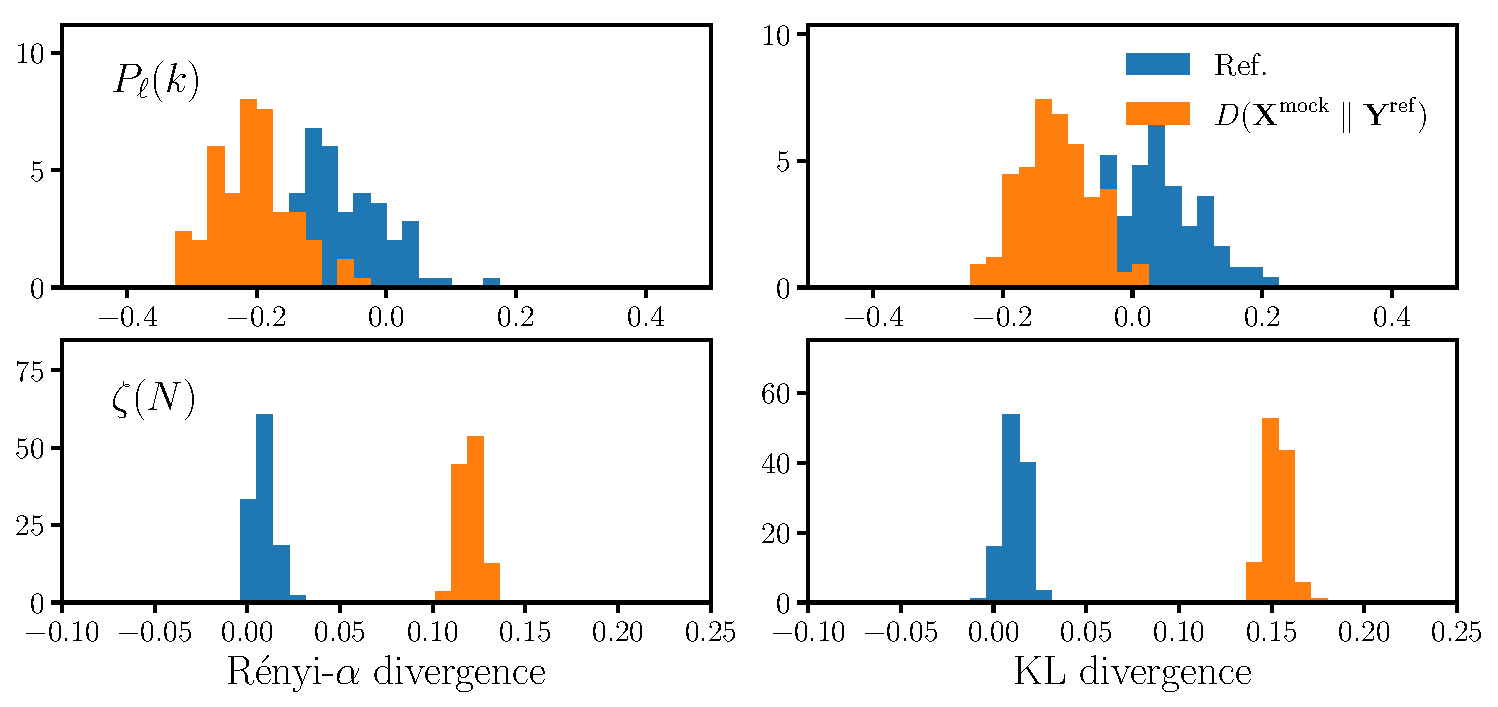
\includegraphics[width=0.9\textwidth]{figs/kNNdiverg_Gauss.pdf}
\caption{R\'enyi-$\alpha$ and KL divergence estimates, ($D_{R\alpha}$ and $D_{KL}$), 
between the mock data ${\bf X}^\mathrm{mock}$ and a reference sample 
${\bf Y}^\mathrm{ref}$ for the $P_\ell(k)$ (left) and $\zeta(N)$ (right) analyses.}
\label{fig:div_gauss}
\end{center}
\end{figure}

\begin{figure}
\begin{center}
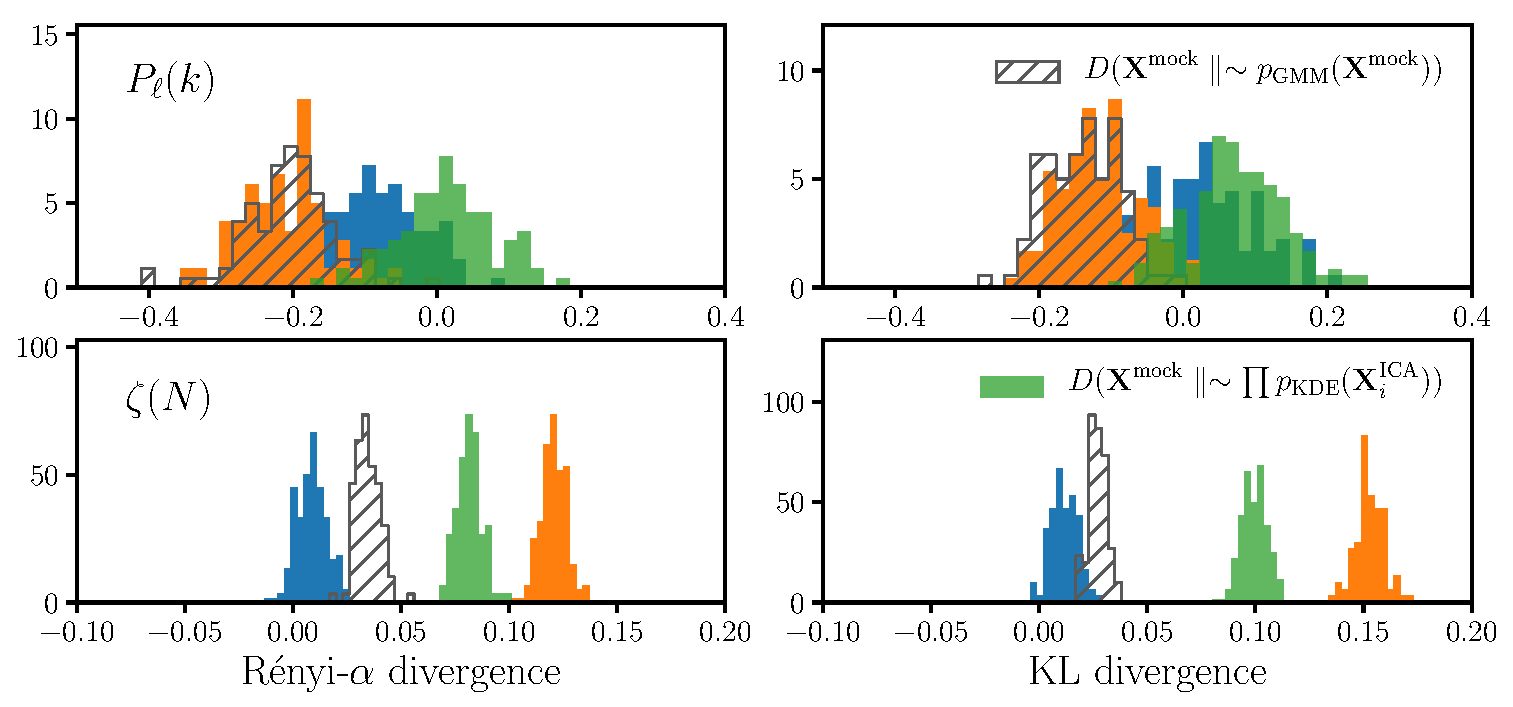
\includegraphics[width=0.9\textwidth]{figs/kNNdiverg_nonGauss.pdf}
\caption{}
\label{fig:div_nongauss}
\end{center}
\end{figure}

\begin{figure}
\begin{center}
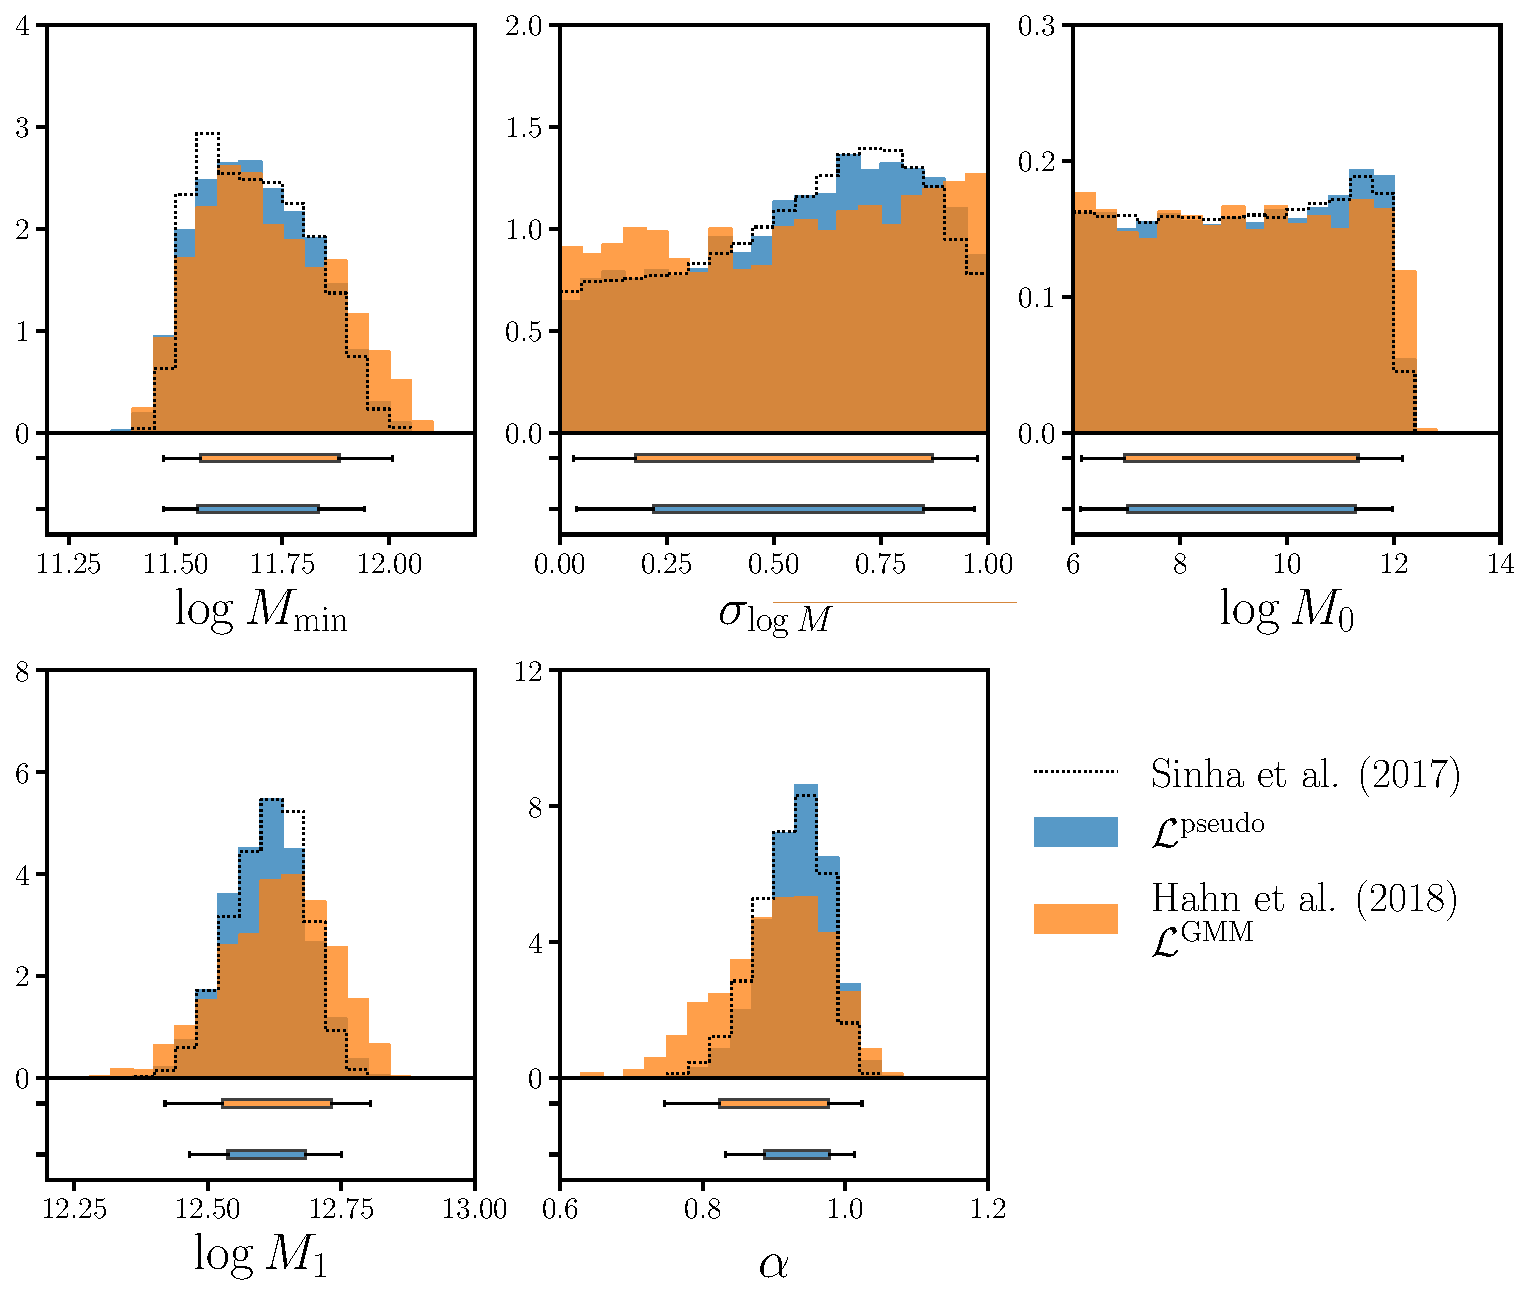
\includegraphics[width=\textwidth]{figs/Like_GMF_comparison.pdf}
\caption{}
\label{fig:gmf_like}
\end{center}
\end{figure}

\begin{figure}
\begin{center}
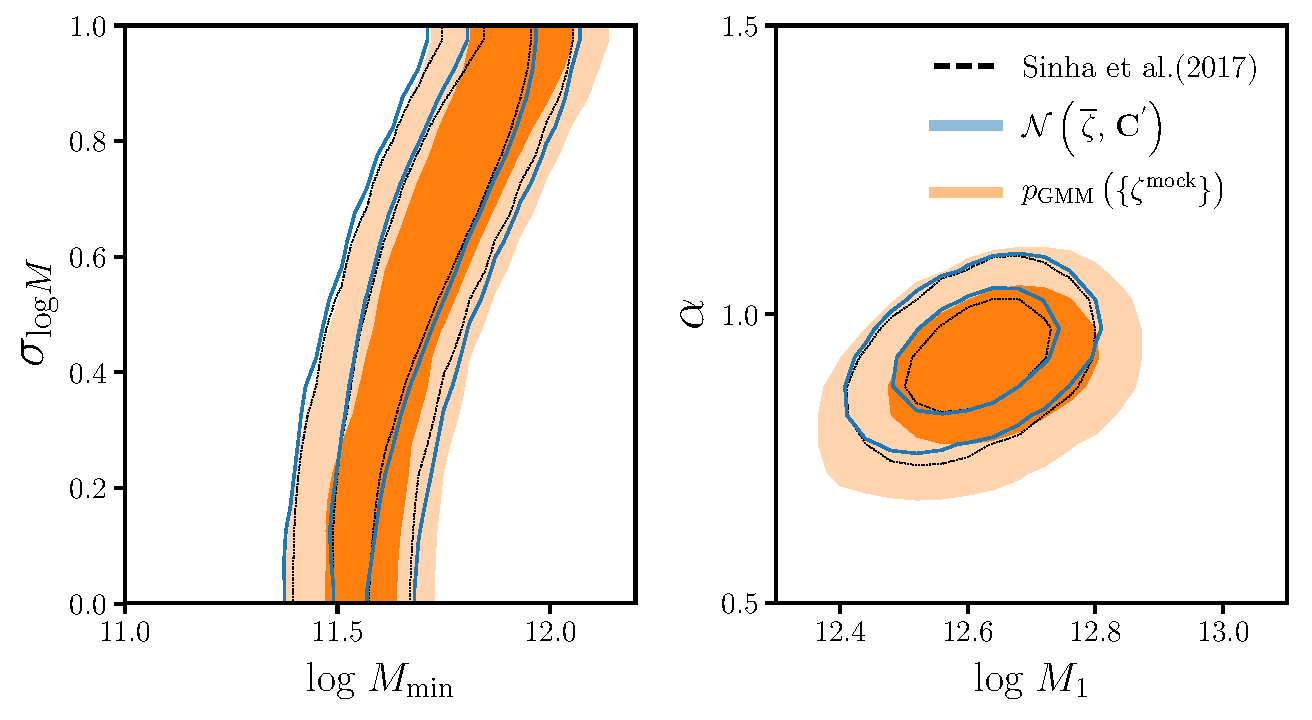
\includegraphics[width=0.9\textwidth]{figs/GMFcontours_manodeep.pdf}
\caption{}
\label{fig:gmf_contour}
\end{center}
\end{figure}

%%%%%%%%%%%%%%%%%%%%%%%%%%%%%%%%%%%%%%%%%%%%%%%%%%%%%%%%%%%%%%%
% Acknowledgements
%%%%%%%%%%%%%%%%%%%%%%%%%%%%%%%%%%%%%%%%%%%%%%%%%%%%%%%%%%%%%%%
\section*{Acknowledgements}
It's a pleasure to thank 
    Simone~Ferraro,
    David~W.~Hogg,
    Emmaneul~Schaan, 
    Roman~Scoccimarro
    Zachary~Slepian

\bibliographystyle{yahapj}
\bibliography{nongausslike}
\end{document}
